\chapter{Química verde e processos industriais}\label{ch:b3:green-industrial}

O ibuprofeno era produzido em seis etapas que descartavam mais massa do que
conservavam: sais de alumínio, cloreto de sódio, etanol, amônia e ácido acético saíam
da fábrica para cada quilograma de fármaco. Desde 1992, uma rota catalítica em três etapas
transforma no produto a maior parte dos átomos que usa, e seu único
subproduto, o ácido acético, é recuperado e vendido. Este capítulo põe números em
comparações desse tipo: \omterm{def:b3:green-industrial:atom-economy}{economia atômica}, \omterm{def:b3:green-industrial:e-factor}{fatores E} e \omterm{def:b3:green-industrial:pmi}{intensidade mássica do processo}; depois
examina os solventes, a energia e a \omterm{def:b3:green-industrial:lca}{avaliação do ciclo de vida}, a maneira como alguns dos maiores
processos químicos se tornaram mais limpos e o que mudam as \omterm{def:b3:green-industrial:feedstock}{matérias-primas renováveis} e as
\omterm{def:b3:complex-kinetics:enzyme}{enzimas}.

\begin{recall}
O volume escolar introduziu a \omterm{def:b3:green-industrial:atom-economy}{economia atômica} e a \omterm{def:b3:green-industrial:green-chemistry}{química verde}; o volume do 1.º
ano, os rendimentos; o volume do 2.º ano, os reatores, a conversão, a seletividade, o tempo
de residência, a conversão por passagem, a reciclagem e a purga, a elevação adiabática de temperatura,
os eletrolisadores e as células a combustível. O \cref{ch:b3:surfaces-catalysis} e o
\cref{ch:b3:homogeneous-catalysis} trataram da catálise, o
\cref{ch:b3:total-synthesis}, das medidas de uma rota sintética.
\end{recall}

\begin{omfigure}
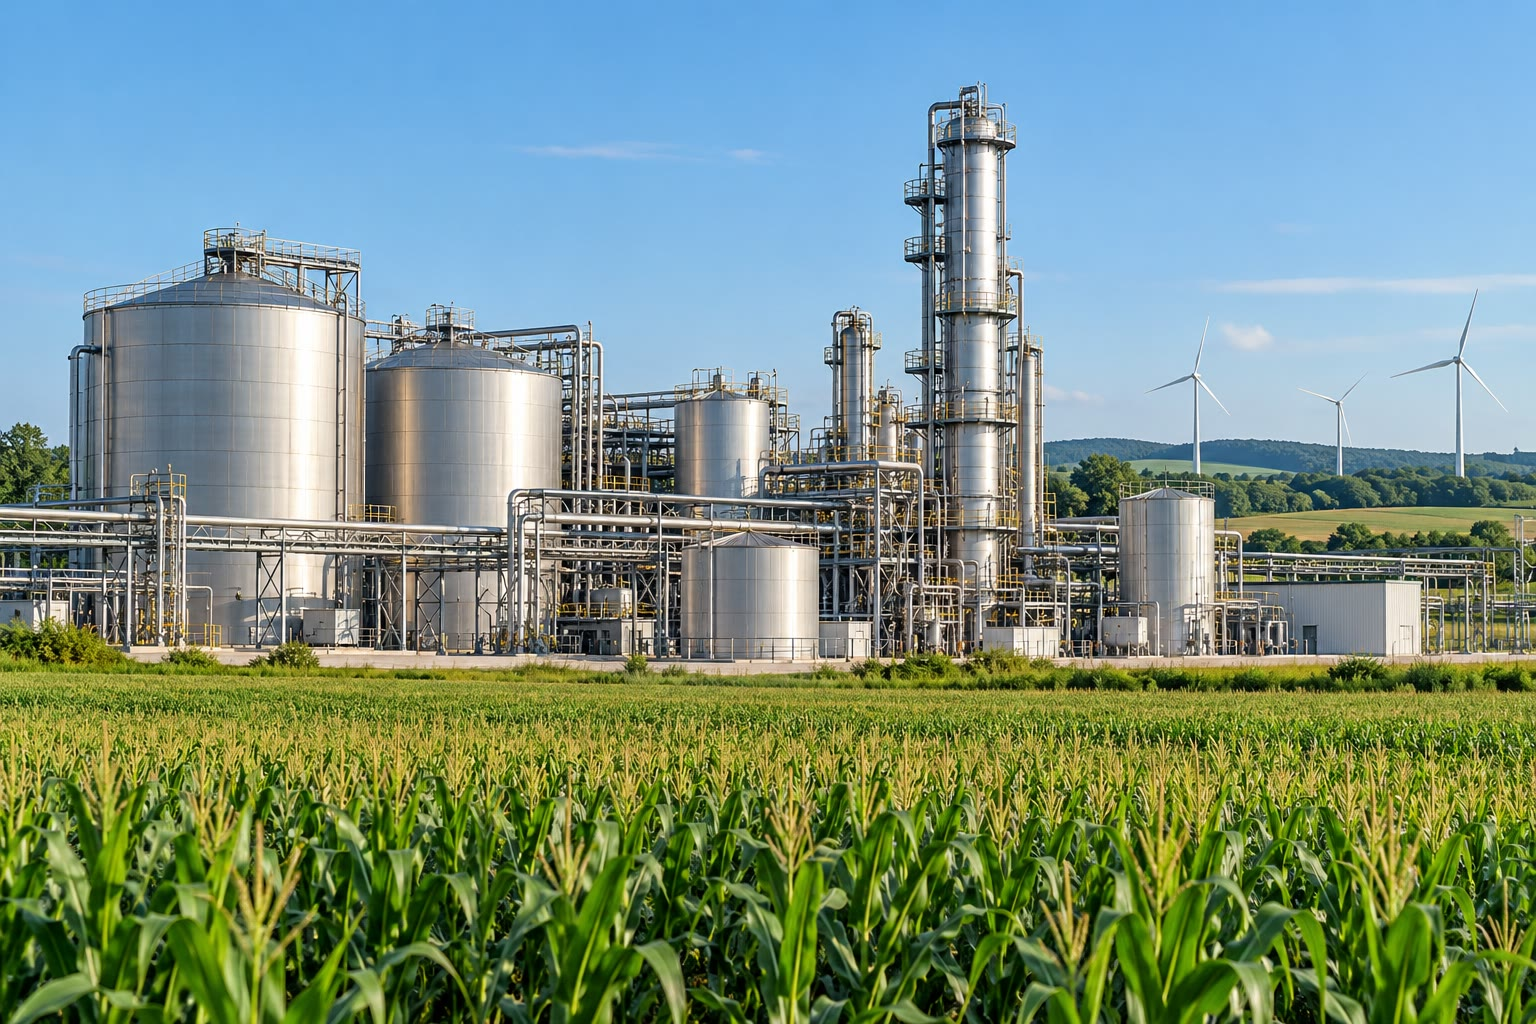
\includegraphics[width=0.58\linewidth]{images/book4/ai/b3-31-biorefinery.jpg}

{\small Uma biorrefinaria: tanques de fermentação e uma coluna de destilação que transformam
culturas e resíduos em combustíveis e em produtos químicos plataforma.}
\end{omfigure}

\section{Medir o caráter verde}

\begin{definition}[Química verde]\label{def:b3:green-industrial:green-chemistry}
A \emph{química verde}\index{quimica verde@química verde} é o planejamento de produtos e
processos químicos que reduzem ou eliminam o uso e a geração de
substâncias perigosas, resumido em doze princípios: prevenir os resíduos, maximizar
a \omterm{def:b3:green-industrial:atom-economy}{economia atômica}, usar e produzir substâncias menos perigosas, planejar produtos mais seguros,
usar solventes mais seguros, economizar energia, usar \omterm{def:b3:green-industrial:feedstock}{matérias-primas renováveis}, evitar derivados
desnecessários, preferir catalisadores a reagentes estequiométricos, planejar para a
degradação, monitorar em tempo real e escolher uma química intrinsecamente mais segura.
\end{definition}

\begin{definition}[Economia atômica]\label{def:b3:green-industrial:atom-economy}
A \emph{economia atômica}\index{economia atomica@economia atômica} de uma reação é a massa molar do
produto desejado dividida pela soma das massas molares de todos os
reagentes da equação balanceada, em porcentagem.
\end{definition}

\begin{proposition}[Economia atômica por classe de reação]\label{prop:b3:green-industrial:ae-classes}
As adições e os rearranjos têm \omterm{def:b3:green-industrial:atom-economy}{economia atômica} de 100\,\%; as substituições e
as eliminações, menos.
\end{proposition}

\begin{proof}
Em uma adição, $\mathrm{A} + \mathrm{B} \to \mathrm{AB}$, ou em um rearranjo, $\mathrm{A} \to \mathrm{A'}$, o único produto contém todos os
átomos dos reagentes, de modo que sua massa molar é igual à soma das deles. Uma
substituição, $\mathrm{A{-}X} + \mathrm{Y} \to \mathrm{A{-}Y} + \mathrm{X}$, ou uma eliminação, $\mathrm{A} \to \mathrm{B} + \mathrm{C}$, produz um
segundo produto que leva massa embora.
\end{proof}

\begin{definition}[Fator E]\label{def:b3:green-industrial:e-factor}
O \emph{fator E}\index{fator E} de um processo é a massa de resíduos por massa de
produto. No fator E completo, todas as entradas que não terminam no produto contam como
resíduo, inclusive os solventes e a água; o fator E simples deixa de fora os solventes e a
água.
\end{definition}

\begin{definition}[Intensidade mássica do processo]\label{def:b3:green-industrial:pmi}
A \emph{intensidade mássica do processo}\index{intensidade massica do processo@intensidade mássica do processo} (PMI) é a
massa total de materiais introduzidos em um processo (reagentes, auxiliares, solventes,
água) por massa de produto.
\end{definition}

\begin{proposition}[PMI e fator E]\label{prop:b3:green-industrial:pmi-e}
Para a mesma fronteira, $\mathrm{PMI} = E + 1$, com $E$ o \omterm{def:b3:green-industrial:e-factor}{fator E} completo.
\end{proposition}

\begin{proof}
Pela conservação da massa, tudo o que entra sai como produto ou como resíduo:
$m_{\mathrm{in}} = m_{\mathrm{product}} + m_{\mathrm{waste}}$. Dividindo por $m_{\mathrm{product}}$, obtém-se $\mathrm{PMI} = 1 + E$.
\end{proof}

\begin{definition}[Eficiência mássica da reação]\label{def:b3:green-industrial:rme}
A \emph{eficiência mássica da reação}\index{eficiencia massica da reacao@eficiência mássica da reação} (RME) de uma
reação é a massa de produto obtida dividida pela massa total dos
reagentes usados.
\end{definition}

\begin{proposition}[RME a partir do rendimento e da economia atômica]\label{prop:b3:green-industrial:rme}
$\mathrm{RME} = \mathrm{AE} \times \text{rendimento}/\mathrm{SF}$, onde o fator estequiométrico $\mathrm{SF} \ge 1$ é a massa de
reagentes usada dividida pela massa que a equação balanceada exige.
\end{proposition}

\begin{proof}
Para um mol de produto esperado, a equação exige uma massa $\sum M_r$ de reagentes e
a operação usa $\mathrm{SF}\sum M_r$; ela dá $\text{rendimento} \times M_{\mathrm p}$ de produto. Dividindo, obtém-se
$\mathrm{RME} = \text{rendimento}\,M_{\mathrm p}/(\mathrm{SF}\sum M_r) = \mathrm{AE} \times \text{rendimento}/\mathrm{SF}$.
\end{proof}

\begin{method}[Calcular as métricas de uma rota]\label{met:b3:green-industrial:metrics}
\begin{enumerate}
  \item Escreva a equação balanceada de cada etapa e calcule a \omterm{def:b3:green-industrial:atom-economy}{economia atômica} da
        rota a partir de todos os reagentes que nela entram.
  \item A partir do registro do lote, some as massas de tudo o que foi carregado (reagentes,
        auxiliares, solventes, água, materiais de isolamento): PMI = total que entra / produto.
  \item $E = \mathrm{PMI} - 1$; subtraia os fluxos recuperados e reutilizados se estiverem dentro da
        fronteira, e diga isso.
  \item RME de cada etapa: produto / reagentes, para descobrir onde o material se perde
        (baixo rendimento, excesso de reagente ou \omterm{def:b3:green-industrial:atom-economy}{economia atômica} ruim).
\end{enumerate}
\end{method}

\begin{omfigure}
\begin{tikzpicture}
\begin{axis}[name=a, width=0.48\linewidth, height=5.4cm, ybar, bar width=14pt, ymin=0, ymax=110,
  xtick={1,2,3,4}, xticklabels={{ibuprofeno, 6 etapas}, {ibuprofeno, 3 etapas}, {OE, cloridrina}, {OE, direta}},
  x tick label style={font=\scriptsize, rotate=25, anchor=north east}, ylabel={economia atômica / \%},
  axis lines=left, tick label style={font=\scriptsize}, label style={font=\small},
  nodes near coords, nodes near coords style={font=\scriptsize, /pgf/number format/fixed, /pgf/number format/precision=0},
  enlarge x limits=0.18]
\addplot[fill=omMeth!55, draw=omMeth] table[x=i, y=AE] {figdata/out/bachelor-3-green-metrics.dat};
\end{axis}
\begin{axis}[at={(a.east)}, anchor=west, xshift=1.4cm, width=0.48\linewidth, height=5.4cm, ybar, bar width=14pt, ymin=0, ymax=3.4,
  xtick={1,2,3,4}, xticklabels={{ibuprofeno, 6 etapas}, {ibuprofeno, 3 etapas}, {OE, cloridrina}, {OE, direta}},
  x tick label style={font=\scriptsize, rotate=25, anchor=north east}, ylabel={fator E mínimo},
  axis lines=left, tick label style={font=\scriptsize}, label style={font=\small},
  nodes near coords, nodes near coords style={font=\scriptsize, /pgf/number format/fixed, /pgf/number format/precision=2},
  enlarge x limits=0.18]
\addplot[fill=omThm!45, draw=omThm] table[x=i, y=Emin] {figdata/out/bachelor-3-green-metrics.dat};
\end{axis}
\end{tikzpicture}

{\small \omterm{def:b3:green-industrial:atom-economy}{Economias atômicas} de duas rotas para o ibuprofeno e de duas rotas para o óxido de etileno
(OE), e os menores \omterm{def:b3:green-industrial:e-factor}{fatores E} que elas permitem (todos os rendimentos de 100\,\%, sem solvente):
$E_{\min} = (1 - \mathrm{AE})/\mathrm{AE}$. Os \omterm{def:b3:green-industrial:e-factor}{fatores E} reais, com rendimentos abaixo de 100\,\%, excessos de reagentes e
solventes, são maiores.}
\end{omfigure}

\section{Solventes e energia}

Os solventes são em geral a maior parte da massa de um processo de química fina ou
farmacêutico. Os guias de seleção de solventes os classificam por critérios de segurança, de saúde e
ambientais: a água, o etanol, o acetato de etila, o 2-metiltetra-hidrofurano
e o anisol são recomendados; o diclorometano, o clorofórmio, o benzeno, o hexano,
a dimetilformamida e o 1,4-dioxano devem ser evitados ou são proibidos. A água,
o dióxido de carbono supercrítico (que dissolve os compostos apolares e não deixa
resíduo quando a pressão é liberada) e as reações sem solvente eliminam o
problema na fonte.

\begin{method}[Usar um guia de seleção de solventes]\label{met:b3:green-industrial:solvent-choice}
\begin{enumerate}
  \item Liste o que o solvente precisa fazer: dissolver os reagentes, resistir aos reagentes,
        ferver a uma temperatura utilizável, separar-se da água no isolamento.
  \item Escolha primeiro na classe recomendada; verifique suas advertências de perigo.
  \item Se um solvente problemático for necessário, procure um recomendado com a mesma
        função (o 2-metiltetra-hidrofurano no lugar do diclorometano ou do THF nas
        extrações, o acetato de etila e o heptano no lugar do hexano em cromatografia).
  \item Planeje sua recuperação por destilação, e conte no \omterm{def:b3:green-industrial:e-factor}{fator E} o que se perde.
\end{enumerate}
\end{method}

\begin{definition}[Intensificação de processos]\label{def:b3:green-industrial:intensification}
A \emph{intensificação de processos}\index{intensificacao de processos@intensificação de processos} é o
reprojeto dos equipamentos e das condições de operação para tornar um processo muito menor,
mais seguro ou mais eficiente: reatores de fluxo contínuo de pequeno volume e
grande área de troca térmica, destilação reativa, aquecimento por micro-ondas.
\end{definition}

Em um reator de fluxo, só existe a cada instante um pequeno volume de um intermediário perigoso,
e o calor é removido muito mais depressa que em um grande recipiente em batelada; reações
que sairiam de controle em um tanque podem ser conduzidas a temperaturas e
concentrações mais altas. Os catalisadores substituem os reagentes estequiométricos, economizando ao mesmo tempo o
reagente e o resíduo em que ele se transforma: a acilação de Friedel--Crafts da antiga
rota do ibuprofeno usava cloreto de alumínio em quantidade estequiométrica, destruído no
isolamento; a nova usa fluoreto de hidrogênio como catalisador e solvente,
recuperado e reutilizado.

\section{O raciocínio em ciclo de vida}

\begin{definition}[Avaliação do ciclo de vida]\label{def:b3:green-industrial:lca}
Uma \emph{avaliação do ciclo de vida}\index{avaliacao do ciclo de vida@avaliação do ciclo de vida} (ACV) avalia os
impactos ambientais de um produto ao longo de sua vida, da extração das matérias-primas
ao descarte. Ela é expressa por \emph{unidade funcional}\index{unidade funcional},
o serviço prestado (por exemplo, uma lavagem de uma carga de roupa), dentro de uma
\emph{fronteira do sistema}\index{fronteira do sistema} que diz quais processos estão
incluídos. Uma \emph{avaliação do berço ao portão}\index{avaliacao do berco ao portao@avaliação do berço ao portão}
termina quando o produto sai da fábrica.
\end{definition}

\begin{omfigure}
\begin{tikzpicture}[font=\scriptsize, >=Stealth,
  box/.style={draw, rounded corners, fill=omDef!10, align=center, minimum height=8mm, inner sep=3pt}]
  \node[box] (r) at (0,0) {extração\\ de recursos\\ naturais};
  \node[box] (p) at (2.6,0) {produção\\ química};
  \node[box] (f) at (5.2,0) {formulação,\\ embalagem};
  \node[box] (u) at (7.8,0) {uso};
  \node[box] (e) at (10.2,0) {fim de vida:\\ reciclagem,\\ descarte};
  \foreach \a/\b in {r/p, p/f, f/u, u/e} \draw[->, thick] (\a) -- (\b);
  \draw[omThm, thick, dashed, rounded corners] (-1.1,-0.75) rectangle (3.75,0.75);
  \node[omThm, anchor=north] at (1.3,-0.8) {fronteira do berço ao portão};
  \draw[omMeth, thick, dashed, rounded corners] (-1.25,-1.35) rectangle (11.5,0.95);
  \node[omMeth, anchor=north] at (5.1,-1.4) {fronteira do berço ao túmulo};
  \node[anchor=south] at (5.1,1.0) {entradas: materiais, energia, água \quad saídas: produto, emissões, resíduos};
\end{tikzpicture}

{\small Etapas da vida de um produto e duas \omterm{def:b3:green-industrial:lca}{fronteiras do sistema}. As entradas e as saídas
são inventariadas para cada processo dentro da fronteira e convertidas em categorias de
impacto (mudança climática, acidificação, uso de água, toxicidade\dots) por
\omterm{def:b3:green-industrial:lca}{unidade funcional}.}
\end{omfigure}

\begin{definition}[Pegada de carbono]\label{def:b3:green-industrial:carbon-footprint}
A \emph{pegada de carbono}\index{pegada de carbono} de um produto é sua
emissão de gases de efeito estufa ao longo do ciclo de vida, expressa como a massa de dióxido de carbono
com o mesmo efeito de aquecimento.
\end{definition}

\begin{method}[Montar uma ACV comparativa]\label{met:b3:green-industrial:lca}
\begin{enumerate}
  \item Enuncie o objetivo e a \omterm{def:b3:green-industrial:lca}{unidade funcional}: compare o que presta o mesmo
        serviço, e não a mesma massa.
  \item Trace a mesma \omterm{def:b3:green-industrial:lca}{fronteira do sistema} para as duas opções.
  \item Inventarie as entradas e as saídas de cada processo dentro dela, com as fontes
        e as datas dos dados.
  \item Converta em categorias de impacto, depois procure os compromissos (menos carbono, mas
        mais água) e teste quão sensível a conclusão é aos dados.
\end{enumerate}
\end{method}

\section{Grandes processos e sua melhoria}

\begin{proposition}[Dióxido de carbono da amônia]\label{prop:b3:green-industrial:smr}
Produzir amônia com hidrogênio obtido pela reforma a vapor do metano libera, apenas pela
matéria-prima, $3/8$ mol de $\ce{CO2}$ por mol de $\ce{NH3}$: cerca de \qty{0.97}{t} de $\ce{CO2}$ por tonelada de amônia.
\end{proposition}

\begin{proof}
A reforma seguida do deslocamento gás-água é, no total, $\ce{CH4 + 2H2O -> CO2 + 4H2}$. A síntese
é $\ce{N2 + 3H2 -> 2NH3}$: dois mols de amônia exigem três de hidrogênio, isto é, $3/4$ mol de
metano e $3/4$ mol de $\ce{CO2}$; por mol de amônia, $3/8$. Uma tonelada de amônia
(\qty{17.0}{g/mol}) corresponde a $\qty{5.88e4}{mol}$, o que dá $\qty{2.21e4}{mol} \times \qty{44.0}{g/mol} = \qty{0.97}{t}$ de $\ce{CO2}$. A queima de metano
para fornecer o calor da reforma acrescenta mais.
\end{proof}

% ledger: nh3:world-2024
As fábricas de amônia, que produzem cerca de 150 milhões de toneladas de nitrogênio por ano, estão entre
as maiores fontes isoladas de dióxido de carbono industrial; o hidrogênio obtido por
eletrólise com eletricidade de baixo carbono, ou a captura de carbono no reformador,
são os caminhos para reduzi-lo. O próprio circuito de amônia, com sua baixa conversão
por passagem, a reciclagem do gás não convertido e a purga do argônio e do metano que
de outro modo se acumulariam, já é eficiente.

\begin{omfigure}
\begin{tikzpicture}[font=\scriptsize, >=Stealth,
  box/.style={draw, rounded corners, fill=omMeth!10, align=center, minimum height=8mm, inner sep=3pt}]
  \node[box] (m) at (0,0) {misturador};
  \node[box] (c) at (2.6,0) {compressor};
  \node[box] (r) at (5.2,0) {conversor\\ (catalisador\\ de ferro)};
  \node[box] (s) at (8.0,0) {condensador,\\ separador};
  \draw[->, thick] (-1.8,0) -- (m) node[pos=0, left, align=right] {$\ce{N2 + 3H2}$\\ (reposição)};
  \draw[->, thick] (m) -- (c); \draw[->, thick] (c) -- (r); \draw[->, thick] (r) -- (s);
  \draw[->, thick] (s) -- ++(0,-1.2) node[below] {$\ce{NH3}$ líquida};
  \draw[->, thick] (s.north) -- ++(0,0.8) -| node[pos=0.25, above] {reciclagem do gás não convertido} (m.north);
  \draw[->, thick, omThm] ($(s.north)+(0,0.8)$) -- ++(1.6,0) node[right] {purga (Ar, $\ce{CH4}$)};
\end{tikzpicture}

{\small O circuito de síntese da amônia: o gás novo é misturado ao gás reciclado,
comprimido e passado sobre o catalisador; a amônia é condensada, o gás não
convertido retorna, e uma pequena corrente de purga remove os gases inertes que
de outro modo se acumulariam.}
\end{omfigure}

Outros grandes processos mostram as mesmas lições. O processo de contato do ácido
sulfúrico é tão exotérmico que uma fábrica moderna exporta vapor e eletricidade.
O óxido de etileno foi primeiro produzido via etilenocloridrina, com cloreto de cálcio
como resíduo; a oxidação direta do etileno com oxigênio sobre prata, uma
adição com 100\,\% de \omterm{def:b3:green-industrial:atom-economy}{economia atômica}, o substituiu, à custa de um pouco de etileno queimado a
dióxido de carbono. O óxido de propileno é hoje produzido também com peróxido de hidrogênio sobre um
catalisador de \omterm{def:b3:inorganic-materials:zeolite}{zeólita} de titânio, com água como único subproduto. O ácido adípico,
produzido pela oxidação do ciclo-hexanol e da ciclo-hexanona com ácido nítrico, libera
óxido nitroso, um forte gás de efeito estufa, que as fábricas hoje destroem cataliticamente.

\section{Matérias-primas renováveis e biocatálise}

\begin{definition}[Matérias-primas renováveis]\label{def:b3:green-industrial:feedstock}
Uma \emph{matéria-prima renovável}\index{materia-prima renovavel@matéria-prima renovável} é uma matéria-prima
reposta em uma escala de tempo humana, como a biomassa vegetal. Uma \emph{molécula
plataforma}\index{molecula plataforma@molécula plataforma} é um composto simples produzido a partir dela em grandes
quantidades e convertido em muitos produtos: etanol, ácido lático, ácido succínico,
glicerol, ácido levulínico, furfural, 5-(hidroximetil)furfural.
\end{definition}

\begin{definition}[Biocatálise]\label{def:b3:green-industrial:biocatalysis}
A \emph{biocatálise}\index{biocatalise@biocatálise} é o uso de \omterm{def:b3:complex-kinetics:enzyme}{enzimas}, isoladas ou em
células, como catalisadores de transformações químicas.
\end{definition}

As \omterm{def:b3:complex-kinetics:enzyme}{enzimas} trabalham em água perto da temperatura ambiente com uma seletividade requintada, e a
evolução dirigida hoje as adapta a substratos não naturais: uma transaminase
evoluída para esse fim substituiu uma hidrogenação assimétrica catalisada por ródio
na fabricação da sitagliptina, um fármaco contra o diabetes, e as cetorredutases produzem muitos
álcoois quirais. O próprio dióxido de carbono é uma matéria-prima: a ureia é produzida a partir dele e da
amônia, e o metanol a partir dele e do hidrogênio. O poli(tereftalato de etileno) pode ser
despolimerizado por glicólise ou metanólise até seus monômeros, ou por
\omterm{def:b3:complex-kinetics:enzyme}{enzimas} modificadas, e repolimerizado.

\begin{inthelab}[Substituir o diclorometano em um isolamento]
Um produto que era extraído da água com diclorometano passa a ser extraído
com 2-metiltetra-hidrofurano: este é produzido a partir de biomassa, separa-se
nitidamente da água (é apenas parcialmente miscível) e forma a camada superior, e não
a inferior, o que muda a ordem das operações no funil de separação. As
camadas orgânicas são secas, o solvente é destilado a pressão reduzida e
recolhido para reutilização.
\end{inthelab}

\begin{safety}{\ghs[0.62cm]{GHS02}\ghs[0.62cm]{GHS04}\ghs[0.62cm]{GHS06}\ghs[0.62cm]{GHS08}}
% ledger: ghs4:EO, ghs:CH2Cl2, ghs4:2MeTHF
Óxido de etileno: gás extremamente inflamável sob pressão, tóxico se inalado, pode
provocar câncer e defeitos genéticos; só existe em sistemas industriais fechados
e em unidades de esterilização. O diclorometano é suspeito de provocar câncer, e o
2-metiltetra-hidrofurano é inflamável e corrosivo para os olhos: um solvente mais verde
não é um solvente inofensivo.
\end{safety}

\begin{history}[Doze princípios e um número]
Paul Anastas e John Warner publicaram os doze princípios da \omterm{def:b3:green-industrial:green-chemistry}{química
verde} em 1998. Roger Sheldon introduziu o \omterm{def:b3:green-industrial:e-factor}{fator E} em 1992, observando que
as indústrias de química fina e farmacêutica, embora pequenas em tonelagem,
produziam muito mais resíduos por quilograma de produto que a química de base. O
processo do ibuprofeno em três etapas, iniciado em 1992, tornou-se um dos primeiros
exemplos da nova abordagem.
\end{history}

\section{Exercícios}

\begin{exercise}[$\star$]\label{exo:b3:green-industrial:1}
Calcule a \omterm{def:b3:green-industrial:atom-economy}{economia atômica} da reação de Diels--Alder do butadieno com o eteno, da
esterificação do ácido acético com o etanol e da reação de Wittig do
benzaldeído com $\ce{Ph3P=CH2}$ (que dá estireno e óxido de trifenilfosfina).
\end{exercise}

\begin{exercise}[$\star$]\label{exo:b3:green-industrial:2}
Um lote usa 120 kg de materiais (reagentes, solventes e água) e dá 8.0 kg de
produto. Calcule a PMI e o \omterm{def:b3:green-industrial:e-factor}{fator E} completo.
\end{exercise}

\begin{exercise}[$\star$]\label{exo:b3:green-industrial:3}
Escolha uma \omterm{def:b3:green-industrial:lca}{unidade funcional} para comparar dois detergentes para roupa e diga por que
``um quilograma de pó'' seria uma má escolha.
\end{exercise}

\begin{exercise}[$\star$]\label{exo:b3:green-industrial:4}
Sugira substitutos mais verdes para o diclorometano em uma extração, o hexano em
cromatografia e a DMF em um acoplamento de amida.
\end{exercise}

\begin{exercise}[$\star\star$]\label{exo:b3:green-industrial:5}
Uma esterificação de 60.0 g de ácido acético com 92.0 g de etanol (o dobro da
quantidade estequiométrica) dá 70.4 g de acetato de etila. Calcule o rendimento, a \omterm{def:b3:green-industrial:atom-economy}{economia
atômica}, o fator estequiométrico e a RME, e verifique a relação entre
eles.
\end{exercise}

\begin{exercise}[$\star\star$]\label{exo:b3:green-industrial:6}
Calcule as \omterm{def:b3:green-industrial:atom-economy}{economias atômicas} das rotas via cloridrina e por oxidação direta para o
óxido de etileno, e a massa de cloreto de cálcio produzida por tonelada de óxido de etileno
pela primeira.
\end{exercise}

\begin{exercise}[$\star\star$]\label{exo:b3:green-industrial:7}
Verifique o $\ce{CO2}$ por tonelada de amônia do capítulo e calcule o $\ce{CO2}$ por tonelada de
hidrogênio produzido por reforma a vapor.
\end{exercise}

\begin{exercise}[$\star\star$]\label{exo:b3:green-industrial:8}
Calcule a energia elétrica mínima, em kWh, para produzir um quilograma de hidrogênio por
eletrólise da água líquida a \qty{25}{\celsius}, a partir de $\Delta_rG^\circ$, e a energia a partir de $\Delta_rH^\circ$.
\end{exercise}

\begin{exercise}[$\star\star$]\label{exo:b3:green-industrial:9}
Se um mol de $\ce{N2O}$ se forma por mol de ácido adípico ($\ce{C6H10O4}$) e o potencial de aquecimento
global do $\ce{N2O}$ é 273 (dados do exercício), calcule o $\ce{N2O}$ e o $\ce{CO2}$ equivalente
por tonelada de ácido adípico sem abatimento.
\end{exercise}

\begin{exercise}[$\star\star\star$]\label{exo:b3:green-industrial:10}
Mostre que, para uma sequência de etapas, a RME global não é o produto das RME das
etapas quando os reagentes em excesso são reciclados, e explique como a reciclagem altera o
\omterm{def:b3:green-industrial:e-factor}{fator E}.
\end{exercise}

\begin{exercise}[$\star\star\star$]\label{exo:b3:green-industrial:11}
Uma melhoria de processo reduz o solvente de uma etapa de 20 L para 5 L por quilograma de
produto (densidade do solvente \qty{0.80}{kg/L}, 90\,\% recuperados por destilação antes e depois; dados
do exercício). Calcule a variação do \omterm{def:b3:green-industrial:e-factor}{fator E} completo.
\end{exercise}

\begin{exercise}[$\star\star\star$]\label{exo:b3:green-industrial:12}
Uma rota de base biológica para um monômero tem menor \omterm{def:b3:green-industrial:carbon-footprint}{pegada de carbono}, mas exige mais terra
e mais água que a rota petroquímica. Como uma ACV comparativa apresentaria isso,
e de que você precisaria para decidir entre elas?
\end{exercise}

\section{Problema: Ibuprofeno, seis etapas ou três?}

\begin{problem}[{Problema de fim de semana --- ibuprofeno, seis etapas ou três:
economias atômicas das duas rotas, fatores E, os catalisadores decisivos e os
resíduos evitados em um ano}]
\label{pb:b3:green-industrial:1}
% ledger: aw:C, aw:H, aw:O, aw:Cl, aw:Na, aw:N
Dados por tonelada de ibuprofeno. Rota em três etapas: 0.71 t de
isobutilbenzeno, 0.55 t de anidrido acético, 0.010 t de hidrogênio, 0.14 t de monóxido
de carbono, 0.05 t de perdas de solvente e catalisador; 0.31 t de ácido acético recuperado
e vendido. Rota em seis etapas: 2.0 t de reagentes e 1.5 t de solventes e auxiliares
não recuperados. Uma fábrica produz 3000 t por ano.

\medskip\noindent\textbf{Parte I --- \omterm{def:b3:green-industrial:atom-economy}{Economia atômica}.}
\begin{enumerate}
  \item Escreva as três etapas da rota catalítica.
  \item Escreva sua equação global.
  \item Calcule as massas molares envolvidas e a \omterm{def:b3:green-industrial:atom-economy}{economia atômica}.
  \item Liste os reagentes da rota em seis etapas (acilação de Friedel--Crafts, condensação
        de Darzens com cloroacetato de etila e etóxido de sódio, hidrólise e
        descarboxilação, formação da oxima, desidratação a nitrila, hidrólise).
  \item Calcule sua \omterm{def:b3:green-industrial:atom-economy}{economia atômica} pela soma das massas molares (com duas águas).
  \item Que subprodutos saem da antiga rota?
\end{enumerate}

\medskip\noindent\textbf{Parte II --- \omterm{def:b3:green-industrial:e-factor}{Fatores E}.}
\begin{enumerate}[resume]
  \item Calcule a massa introduzida na nova rota por tonelada de produto.
  \item Calcule sua PMI e seu \omterm{def:b3:green-industrial:e-factor}{fator E} completo, com o ácido acético contado como resíduo.
  \item Calcule o \omterm{def:b3:green-industrial:e-factor}{fator E} se o ácido acético recuperado for contado como produto.
  \item Calcule a PMI e o \omterm{def:b3:green-industrial:e-factor}{fator E} da antiga rota.
  \item Por que o \omterm{def:b3:green-industrial:e-factor}{fator E} real é maior que $(1 - \mathrm{AE})/\mathrm{AE}$?
  \item Que princípios, entre os doze, as diferenças ilustram?
\end{enumerate}

\medskip\noindent\textbf{Parte III --- Catalisadores.}
\begin{enumerate}[resume]
  \item O que o fluoreto de hidrogênio substitui na acilação, e por que isso importa?
  \item O que catalisa a hidrogenação da cetona ao álcool?
  \item O que catalisa a \omterm{def:b3:homogeneous-catalysis:carbonylation}{carbonilação} do álcool, e de que capítulo é essa química?
  \item Por que o ácido acético é um subproduto nas duas rotas?
  \item Que perigos a nova rota traz, e como eles são gerenciados?
  \item Por que menos etapas significam também menos energia?
\end{enumerate}

\medskip\noindent\textbf{Parte IV --- Um ano.}
\begin{enumerate}[resume]
  \item Calcule os resíduos da antiga rota para a produção anual da fábrica.
  \item Calcule os da nova rota (ácido acético vendido).
  \item Calcule os resíduos evitados por ano.
  \item Um \omterm{def:b3:green-industrial:e-factor}{fator E} menor significa sempre um impacto ambiental menor?
  \item O que uma \omterm{def:b3:green-industrial:lca}{avaliação do ciclo de vida} acrescentaria?
  \item Enuncie o resultado: a \omterm{def:b3:green-industrial:atom-economy}{economia atômica} da rota em três etapas.
\end{enumerate}
\end{problem}
